%%%%%%%%%%%%%%%%%%%%%%%%%%%%%%%%%%%%%%%%%
% Simple Sectioned Essay Template
% LaTeX Template
%
% This template has been downloaded from:
% http://www.latextemplates.com
%
% Note:
% The \lipsum[#] commands throughout this template generate dummy text
% to fill the template out. These commands should all be removed when 
% writing essay content.
%
%%%%%%%%%%%%%%%%%%%%%%%%%%%%%%%%%%%%%%%%%

%----------------------------------------------------------------------------------------
%	PACKAGES AND OTHER DOCUMENT CONFIGURATIONS
%----------------------------------------------------------------------------------------

\documentclass[hidelinks, 12pt]{article} % Default font size is 12pt, it can be changed here

\usepackage{geometry} % Required to change the page size to A4
%\geometry{a4paper} % Set the page size to be A4 as opposed to the default US Letter

\usepackage{graphicx} % Required for including pictures
\usepackage{float} % Allows putting an [H] in \begin{figure} to specify the exact location of the figure
\usepackage{wrapfig} % Allows in-line images such as the example fish picture
\usepackage{setspace} % To control linespacing
\usepackage{enumerate} % For enumerating lists
\usepackage{enumitem} % more enumerating stuff
\usepackage{multicol} % for multicoumn formating
\usepackage{multirow} % for multicoumn formating
\usepackage{adjustbox}
\usepackage{changepage}
\usepackage{fancyhdr}
\usepackage[usenames,dvipsnames]{xcolor} %To change text colors, color options located at: http://en.wikibooks.org/wiki/LaTeX/Colors
\usepackage[font={footnotesize}]{caption}
\usepackage[labelfont=bf]{caption}
\usepackage{longtable}
\usepackage{tabularx}
\usepackage{arydshln}
\usepackage{titlesec} % To control section colors
\usepackage{color}
\usepackage{hyperref} % for web links
\usepackage[toc, acronym, nopostdot, nonumberlist]{glossaries}
\makeglossaries

\graphicspath{{Pictures/}} % Specifies the directory where pictures are stored

\linespread{1.2} % Line spacing
\widowpenalty=8999 
\clubpenalty=8999 

%%%%% Define PSU official colors
\definecolor{PSUgreen}{RGB}{106,127,16}
\definecolor{PSUltgreen}{RGB}{168,180,0}
\definecolor{PSUblue}{RGB}{0,117,154}
\definecolor{PSUltblue}{RGB}{161,216,224}
\definecolor{PSUgray}{RGB}{71,67,52}
\definecolor{PSUBrown}{RGB}{96,53,29}
\definecolor{PSUsienna}{RGB}{163,63,31}
\definecolor{PSUred}{RGB}{210,73,42}
\definecolor{PSUorange}{RGB}{220,155,50}
\definecolor{PSUyellow}{RGB}{230,220,143}
\definecolor{PSUtan}{RGB}{232,221,162}
\definecolor{PSUpurple}{RGB}{101,3,96}

%----------------------------------------------------------------------------------------
%  Section Colors
%----------------------------------------------------------------------------------------
\titleformat{\section}
{\color{PSUgreen}\normalfont\Large\bfseries}
{\color{PSUgreen}\thesection}{1em}{}

\titleformat{\subsection}
{\color{PSUblue}\normalfont\large\bfseries}
{\color{PSUblue}\thesubsection}{1em}{}

\titleformat{\subsubsection}
{\color{PSUblue}\normalfont\normalsize\bfseries}
{\color{PSUblue}\thesubsubsection}{1em}{}

\titleformat{\subparagraph}
{\color{PSUblue}\normalfont\normalsize\bfseries}
{\color{PSUblue}\thesubsubsection}{1em}{}

%----------------------------------------------------------------------------------------
%  Watermark
%----------------------------------------------------------------------------------------
%\usepackage{draftwatermark} % for watermarks
%\SetWatermarkText{\textbf{DRAFT}}
%\SetWatermarkScale{5}
%\SetWatermarkColor[gray]{0.9}
%----------------------------------------------------------------------------------------
%----------------------------------------------------------------------------------------
%	SECTION TABLES MORE THAN ONE LINE IN A CELL
%----------------------------------------------------------------------------------------
\usepackage{makecell}

\renewcommand\theadalign{bc}
\renewcommand\theadfont{\bfseries}
\renewcommand\theadgape{\Gape[4pt]}
\renewcommand\cellgape{\Gape[4pt]}



\begin{document}
\pagestyle{fancy}


%----------------------------------------------------------------------------------------
%	TITLE PAGE
%----------------------------------------------------------------------------------------

\begin{titlepage}
\newcommand{\HRule}{\rule{\linewidth}{0.5mm}} % Defines a new command for the horizontal lines, change thickness here
\center % Center everything on the page

% \HRule \\[0.4cm]
{ \huge \bfseries Power Lab Notebook \\[0.4cm] } % Title of your document
\HRule \\[1.5cm]



\begin{minipage}{0.4\textwidth}
\large
\emph{Authors:}\\
\textsc{Midrar Adham}\\

%{\large \today} % Date
{\large September 11, 2021} 
%\includegraphics{Logo}\\[1cm] % Include a department/university logo - this will require the graphicx package
\end{minipage}\\[0.5cm]
\vfill % Fill the rest of the page with whitespace

\includegraphics[width=3.5in]{psuMCECSlogo_horiz.png}
\vfill
% \textsc{\color{PSUgray}\normalsize Support provided by: \\ Portland General Electric}\\[0.5cm] % Major heading such as course name

\end{titlepage}

%----------------------------------------------------------------------------------------
%	Header
%----------------------------------------------------------------------------------------
\fancyhf{}  % clears the default page numbering
\fancyhead[L]{\footnotesize{\textcolor{PSUgray}{PowerLab Notebook}}}
%\fancyhead[C]{\footnotesize{center head}}
\fancyhead[R]{\footnotesize{\textcolor{PSUgray}{PSU-PowerLab}}}
%----------------------------------------------------------------------------------------
%    Footer
%----------------------------------------------------------------------------------------
%\patchcmd{\footrule}{\hrule}{\color{PSUgreen}\hrule}{}{}
\renewcommand{\footrulewidth}{0.4pt}
\fancyfoot[L]{\footnotesize\color{PSUgray}\sffamily
1900 SW 4$^{th}$ Ave, suite 160, Portland, OR 97201 \textbullet\ \href{http://www.pdx.edu/power-lab/}{www.pdx.edu/power-lab/}}
%\fancyfoot[C]{~}
\fancyfoot[R]{\footnotesize~\newline\color{PSUgray}\sffamily\thepage}
%----------------------------------------------------------------------------------------
%    Section: Abstract
%----------------------------------------------------------------------------------------
% \newpage
% \section*{Abstract}
% \label{Abstract}
% \input{Section_Abstract}
% \pagebreak

%----------------------------------------------------------------------------------------
%    TABLE OF CONTENTS
%----------------------------------------------------------------------------------------
\setcounter{tocdepth}{2}
\tableofcontents % Include a table of contents
%\setlength{\parskip}{3ex plus 2ex minus 2ex}

%----------------------------------------------------------------------------------------
%    Section: List of Figures, Tables, and Glossary
%----------------------------------------------------------------------------------------
\newpage
\listoffigures

\newpage
\listoftables

\printglossary[type=\acronymtype]%----------------------------------------------------------------------------------------
%    Section: Introduction
%----------------------------------------------------------------------------------------
\newpage
\section{Fall 2020}
\label{Fall2020}
\textbf{Water heater object GLD Dec 19, 2020}
\subsection{objective}

    
    Test water heater behavior in GridLAB-D.
    
\subsection{outline}
    
    Using GridLAB-D, a water heater behavior is tested using the following parameter:
\subsection{procedures}
    
    To achieve the goal of this sprint, IEEE$\_$4$\_$Node$\_$Feeder is used. The following objects are needed:
    \begin{itemize}
        \item Triplex objects such as transformers, lines, meter, and water heater.
        \item Water heater parent. Typically a house object.
        \item Water heater object.
    \end{itemize}
    
\subsection{parameters}
    
    \begin{itemize}
        \item Setpoint 120F
        \item Deadband 2F
        \item Volume 50 Gallons
        \item Water demand ELCAP data
        \item heat$\_$mode ELECTRIC
    \end{itemize}
    
\subsection{Data}
    glm file can be found here \par  \url{https://github.com/psu-powerlab/GridLab-D/blob/master/NeoChargeProject/WH_4_Node_Feeder/Uncontrolled_WH/WH_4_node.glm}

    \par Full output data is uploaded to PSU power lab GitHub account, GridLAB-D repository.
    
    \url{https://github.com/MidrarAdham/GridLab-D/blob/master/NeoChargeProject/WH_4_Node_feeder/Water_heater/wh_1.csv}
\newpage
\subsection{results}
        \begin{figure}[hbt!]
            \includegraphics[scale=0.5]{Pictures/controlled_WH.png}
            \caption{Power and Water Demand vs Time (un-controlled)}
            \label{fig:uncontrolled_wh}
        \end{figure}

\newpage
% \pagebreak

%	Section: Conclusion
%----------------------------------------------------------------------------------------
\newpage
\section{Winter 2021}
\label{Winter2021.tex}
\textbf{Control Water heater using switch and passive controller in IEEE 4 node feeder Jan 06, 2021}
\subsection{objective} 
    \begin{itemize}
        \item Test behavior of water heater when controlled by switch object using NR and FBS solvers.
        \item Test water heater behavior when controlled by passive controller.
        \item Test water heater behavior when shed command is received.
        % \item When switch is open, the water heater SHALL not consume watts, however, water temperature SHALL decrease.
        % \item When switch is closed, water heater SHALL behave normally.
    \end{itemize}
\subsection{outline}
    
    What steps are required?
    \begin{enumerate}
        \item Switch Object
        \begin{itemize}
            \item Set up a switch object in 4 node feeder.
            \item Use player object to control the state of the switch (OPEN OR CLOSED).
            \item Define player object timestamp to be compatible with CLOCK object. 
        \end{itemize}
        \item Passive Controller:\par
        Passive controller utilizes energy market. When prices are high, water heater turns OFF. When prices are low, water heater turns ON.
        \begin{itemize}
            \item Set up auction object.
            \item Set up passive controller.
            \item Set up water heater object as passive controller child.
            \item Set up a .player file so auction object can read from it. (Alternative solution: Prices can be scheduled using schedule object.)
        \end{itemize}
        \item Shed Command:
        \begin{itemize}
            \item Change water heater setpoints during simulation to simulate shed command.
        \end{itemize}
    \end{enumerate}
\subsection{procedures}
    \begin{enumerate}
        \item Switch Object
        \begin{itemize}
            \item switch object is placed in the triplex section of the feeder (between center tapped transformer and triplex node).
            \item Remember, switch object SHALL be placed between link-based nodes. 
            \item Switch object SHALL be used in INDIVIDUAL mode. It won't work with BANKED mode.
            \item Use NR solver. Switch object may behave incorrectly with FBS solver.
        \end{itemize}
        \item Passive Controller:
        \begin{itemize}
            \item Import market module
            \item Set up auction object with prices source file.
            \item Set up a player object that contains prices data. This object is auction object child.
            \item Set up 
        \end{itemize}
        \item Shed command:
        \begin{itemize}
            \item Using schedule object, setpoints are scheduled every 10 minutes.
            \item The water temperature SHALL decrease below the original setpoints. 
        \end{itemize}
    \end{enumerate}
\subsection{parameters}
    \begin{enumerate}
        \item Water Heater parameter (without Shed command):
        \begin{itemize}
        \item Setpoint 120F
        \item Deadband 2F
        \item Volume 50 Gallons
        \item Water demand ELCAP data
        \item heat$\_$mode ELECTRIC
        \end{itemize}
        \item Switch object state:
            \begin{itemize}
                \item At 4:00 pm, switch is CLOSED until 6:00 pm.
                \item Switch state changes to OPEN from 6:05 pm until 8:00 pm.
                \item Switch state changes to CLOSED from 8:05 pm until the end of the simulation.
            \end{itemize}
        \item passive$\_$controller:
            \begin{itemize}
                \item period 600 seconds. (This property SHALL match simulation time)
                \item Control$\_$mode PROBABILITY$\_$OFF. (SHALL be used when der is aggregated.)
                \item comfort$\_$level SHALL be set to a high number to force water heater to turn OFF at specified times.
                \item state$\_$ property SHALL be override. This is important to force water heater object to stick to parent object parameter.
            \end{itemize}
    \end{enumerate}
\subsection{observations}
    \begin{enumerate}
        \item Switch object:
        \begin{itemize}
            \item Water heater did not respond to switch changes with NR solver.
            \item When switch is open, water heater still turns ON and consume power (kW).
    \end{itemize}
        \item passive$\_$controller:
        \begin{itemize}
            \item water heater behaves as expected.
        \end{itemize}
        \item shed$\_$command
        \begin{itemize}
            \item Setpoints changed as expected.
        \end{itemize}
    \end{enumerate}
\newpage
    
\subsection{data}
    \begin{enumerate}
        \item Switch$\_$object:
        
    
\begin{table}[h]
\begin{tabular}{|l|l|l|l|l}

\cline{1-4}
Timestamp & power (kW) & water$\_$demand (gpm) & is$\_$waterheater$\_$on & \\ \cline{1-4}
2020-01-01 18:00:00 PST & +0 & +0 & 0 & \\ \cline{1-4}
2020-01-01 18:10:00 PST & 0 & 0.16 & 0 &  \\ \cline{1-4}
2020-01-01 18:20:00 PST & 4.5 & 0 & 1 &  \\ \cline{1-4}
\end{tabular}
\caption{Water heater controlled by a switch}
\label{table:1}
\end{table}
        \item passive$\_$controller \newline
        glm file can be found here: \url{https://github.com/psu-powerlab/GridLab-D/blob/master/NeoChargeProject/WH_4_Node_Feeder/Controlled_WH/Controlled_WH_4.glm} \newline \par
        
        Full output file is uploaded to power lab github account: \url{https://github.com/psu-powerlab/GridLab-D/blob/master/NeoChargeProject/WH_4_Node_Feeder/Controlled_WH/wh_1.csv}
        
        \begin{table}[h]
        \begin{tabular}{|l|l|l|l|l}
        \cline{1-4}
        Timestamp & power (kW) & water$\_$demand (gpm) & is$\_$waterheater$\_$on & \\ \cline{1-4}
        2020-01-01 16:00:00 PST & +0 & +0 & 0 & \\ \cline{1-4}
        2020-01-01 16:10:00 PST & +0 & +0 & 0 &  \\ \cline{1-4}
        2020-01-01 16:20:00 PST & +0 & +0 & 0 &  \\ \cline{1-4}
        2020-01-01 16:30:00 PST & +0 & +0 & 0 &  \\ \cline{1-4}
        2020-01-01 16:40:00 PST & +0 & +0 & 0 &  \\ \cline{1-4}
        2020-01-01 16:50:00 PST & +0 & +0.25 & 0 &  \\ \cline{1-4}
        \end{tabular}
        \caption{Water heater controlled by passive controller}
        \label{table:2}
        \end{table}
        
        \item shed$\_$command \newline
        glm file can be found here \url{https://github.com/psu-powerlab/GridLab-D/blob/master/NeoChargeProject/WH_4_Node_Feeder/Controlled_WH/WH_Shed_command.glm} \newline \par
         Full data is uploaded to PSU power lab GitHub account \url{https://github.com/psu-powerlab/GridLab-D/blob/master/NeoChargeProject/WH_4_Node_Feeder/Controlled_WH/wh_shed.csv}\newline \par Does the shed command contain starting and ending time? 
        
        \begin{table}[h]
        \begin{tabular}{|l|l|l|l|l|l}
        \cline{1-5}
        Timestamp & power (kW) & water$\_$demand (gpm) & water$\_$temperature (F) & is$\_$waterheater$\_$on & \\ \cline{1-5}
        2020-01-01 18:00:00 PST & 0 & 0 & 119.008 & 0 & \\ \cline{1-5}
        2020-01-01 18:10:00 PST & 0 & 0.16 & 118.944 & 0 &  \\ \cline{1-5}
        2020-01-01 18:20:00 PST & 0 & 0 & 117.026 & 0 &  \\ \cline{1-5}
        2020-01-01 18:30:00 PST & 0 & 0 & 116.965 & 0 &  \\ \cline{1-5}
        2020-01-01 18:40:00 PST & 0 & 0 & 116.904 & 0 &  \\ \cline{1-5}
        2020-01-01 18:50:00 PST & 0 & 0 & 116.843 & 0 &  \\
        \cline{1-5}
        \end{tabular}
        \caption{Water heater controlled with shed command}
        \label{table:3}
        \end{table}
    \end{enumerate}
\subsection{results}
    \begin{enumerate}
        \item switch$\_$object

        The above table \ref{table:1} is a portion of the water heater output file. At the specified timestamps, the switch is open. It can be seen from the last row that the water heater was turned ON and consumed 4.5 kW even though switch was open. I sent a request to GridLAB-D folks regarding this issue. I will resume this work on switch object once I receive a response. Alternatively, a passive controller object was used. The results are shown in table \ref{table:2}.
    
        \item passive$\_$controller
        
        A shed command is received at 17:00. The water heater is supposed to turn ON at 18:20 as the water temperature drops below the range (118F). Due to shed command, the water temperature continues to drop as shown in table \ref{table:3}.
        \begin{figure}[hbt!]
            \includegraphics[scale=0.5]{controlled_WH.png}
            \caption{Power and Water Demand vs Time (controlled)}
            \label{fig:controlled_wh}
        \end{figure}
        \newpage
        \item shed$\_$command
        Refer to powerLab github account for glm file and procedure in this link \href{https://github.com/MidrarAdham/GridLab-D/tree/master/NeoChargeProject/WH_4_Node_feeder/WH_shed_command}{Shed Command in EWH}.
        
    \end{enumerate}
    \newpage

\pagebreak
%----------------------------------------------------------------------------------------
%   Section: DCS and CTA-2045
%----------------------------------------------------------------------------------------
\newpage
\section{Spring 2021}
\label{Spring2021}
\textbf{Control Heat Pump Water heater using switch and passive controller in IEEE 4 node feeder Apr 10, 2021}
\subsection{objective} 
    \begin{itemize}
        \item Test behavior of HPWH.
        \item Test HPWH behavior when controlled by passive controller.
    \end{itemize}

\subsection{outline}
    
    What steps are required?
    \begin{enumerate}
        \item Build a WH object with HEAT$\textunderscore$PUMP specified as a heat$\textunderscore$mode.
        \item Passive Controller:\par
        Passive controller utilizes energy market. When prices are high, water heater turns OFF. When prices are low, water heater turns ON.
        \begin{itemize}
            \item Set up auction object.
            \item Set up passive controller.
            \item Set up water heater object as passive controller child.
            \item Set up a .player file so auction object can read from it. (Alternative solution: Prices can be scheduled using schedule object.)
        \end{itemize}
        \item Shed Command:
        \begin{itemize}
            \item Change water heater setpoints during simulation to simulate shed command.
        \end{itemize}
    \end{enumerate}
\subsection{procedures}
    \begin{enumerate}
        \item HP$\textunderscore$WH
        \begin{itemize}
            \item HP$\textunderscore$WH is linked to a house object (Required) as a child.
            \item Need to specify the parent in the WH object. (parent House1;) 
        \end{itemize}
        \item Passive Controller:
        \begin{itemize}
            \item Import market module
            \item Set up auction object with prices source file.
            \item Set up a player object that contains prices data. This object is auction object's child.
        \end{itemize}
        \item Shed command:
        \begin{itemize}
            \item Using schedule object, setpoints are scheduled every 10 minutes.
            \item The water temperature SHALL decrease below the original setpoints. 
        \end{itemize}
    \end{enumerate}
\subsection{parameters}
    \begin{enumerate}
        \item Water Heater parameter (without Shed command):
        \begin{itemize}
        \item Setpoint 120F
        \item Deadband 2F
        \item Volume 50 Gallons
        \item Water demand ELCAP data
        \item heat$\_$mode ELECTRIC
        \end{itemize}
        \item Switch object state:
            \begin{itemize}
                \item At 4:00 pm, switch is CLOSED until 6:00 pm.
                \item Switch state changes to OPEN from 6:05 pm until 8:00 pm.
                \item Switch state changes to CLOSED from 8:05 pm until the end of the simulation.
            \end{itemize}
        \item passive$\_$controller:
            \begin{itemize}
                \item period 600 seconds. (This property SHALL match simulation time)
                \item Control$\_$mode PROBABILITY$\_$OFF. (SHALL be used when der is aggregated.)
                \item comfort$\_$level SHALL be set to a high number to force water heater to turn OFF at specified times.
                \item state$\_$ property SHALL be override. This is important to force water heater object to stick to parent object parameter.
            \end{itemize}
    \end{enumerate}
\subsection{observations}
    \begin{enumerate}
        \item HP$\textunderscore$WH:
        \begin{itemize}
            \item Water temperature increases above the setpoint. HP$\textunderscore$WH object does \textbf{NOT} respond to setpoints as shown in figure \ref{fig:HPWH}.
    \end{itemize}
    \end{enumerate}
    \begin{figure}[htp!]
        \centering
        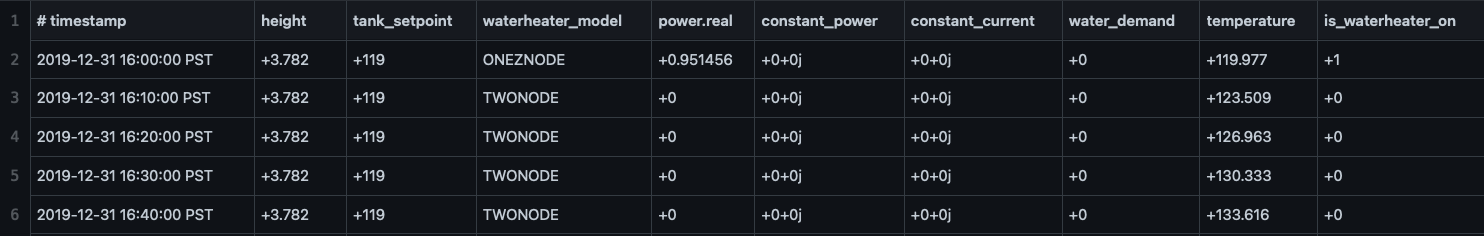
\includegraphics[width=1.1\columnwidth]{Pictures/HPWH_wrong_behavior.png}
        \caption{HPWH object in GLD does not respond to specified setpoints}
        \label{fig:HPWH}
    \end{figure}
    \begin{itemize}
        \item Comparing the HPWH behavior to the EWH, we can see the issue clearly. Figure \ref{fig:EWH} shows the EWH behavior under the same parameters.
    \end{itemize}
    \begin{figure}[htp!]
        \centering
        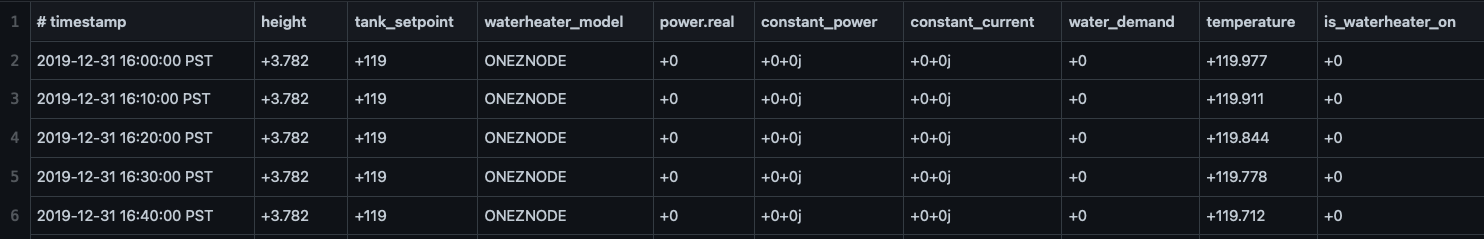
\includegraphics[width=1.1\columnwidth]{Pictures/EWH.png}
        \caption{EWH object in GLD responds properly to specified setpoints}
        \label{fig:EWH}
    \end{figure}
\newpage
    
\subsection{debugging}
\subsubsection{Related links}
\begin{itemize}
    \item Here's my conversation with Frank Tuffner, a GridLAB-D developer, regarding the HPWH. \href{https://sourceforge.net/p/gridlab-d/discussion/842562/thread/4a543d83a0/?limit=25#71e9}{Frank's input regarding HPWH issue.}
    \item On your computer, go to GLD folder $>$ residential $>$ open waterheater.cpp file.
\end{itemize}
\subsection{Water Heater Dynamic Driving Parameters}
\begin{itemize}
    \item Demand
    \begin{itemize}
        \item The higher the demand, the more quickly the thermocline drops.
    \end{itemize}
    \item Voltage
    \begin{itemize}
        \item The line voltage of the coil. The lower the voltage, the more slowly the thermocline rises.
    \end{itemize}
    \item Inlet water temperature
    \begin{itemize}
        \item The lower the inlet water temperature, the more heat needed to raise the temperature to the setpoint.
    \end{itemize}
    \item Indoor air temperature
    \begin{itemize}
        \item The higher the indoor temperature, the less heat loss through the jacket.
    \end{itemize}
\end{itemize}
\subsection{Heating Element Capacity}
The heating element capacity equation in the EWH is voltage dependant as shown in equation \ref{equ:HEC_EWH}.
\begin{equation}
    test = HeatingElementCapacity *(ActualVoltage)^2 / (NominalVoltage)^2
    \label{equ:HEC_EWH}
\end{equation}
However, the heating element capacity for the heat pump water heater does not have a voltage dependence as shown in equation \ref{equ:HEC_HPWH}.
\begin{equation}
    HeatingElementCapacity = (1.09 + (1.17 - 1.09) * (get_Tambient(location) -50) / (70 - 50)) * (0.379 + 0.00364 * Tw)
    \label{equ:HEC_HPWH}
\end{equation}

\subsection{Commented commands by GLD folks}
\begin{itemize}
    \item Heating element capacity (line 1634)
    \item Water temperature increment for onenode and twonode analysis (lines 1656 and 1684)
    \item Coesfficient of Performance (CoP) line 1731
\end{itemize}
\subsection{Water Heater Source Code Structure}
\begin{itemize}
    \item The code is defined by parameters instead of water heater models. 
    \item Some parameters, such as tank$\textunderscore$area, tank$\textunderscore$volume, tank$\textunderscore$height, etc are global as they work with all water heater models (i.e Electric, heat pump, and gas).
    \item Other parameters, such as heating element, need to be calculated when using Heat pump water heater model. The heating element in heat pump water heater is used as a backup.
\end{itemize}
\subsection{Errors Summary}
Running the HPWH object in GLD, we see the following errors:
\begin{itemize}
    \item The property is$\textunderscore$waterheater$\textunderscore$on is randomly 1 or 0. For a correct HPWH behavior, it should be 1 when there's sufficient water demand. Otherwise, it should always be zero.
    \item The waterheater$\textunderscore$model property should be ONEZNODE when there is no water demand. When there is water demand, there is inlet water pumped inside the tank. Therefore, both heating element capacity (top and bottom) should turn on. When both heating element capacity are on, the model switches to TWONODE model which is not the case in the HPWH. Refer to figure \ref{fig:EWH} and figure \ref{fig:HPWH} for a visual analysis.
\end{itemize}
\subsection{Questions}
\begin{itemize}
    \item I know the heating element is used as a backup in the HPWH. How is “backup” defined? Is it used where there’s a high water demand? How high should the water demand be to turn on the heating element?
    \begin{itemize}
        \item There are four modes in the A. O Smith units \cite{r1}. These modes are listed as shown below:
        \begin{itemize}
            \item \textbf{Hybrid Mode:}
            \begin{itemize}
                \item This mode uses the dead-band algorithm. If the average tank temperature (the weighted temperature of the upper and lower thermostat) drops below 9F below the setpoint, then the HP turns on to heat the water.
                \item If the HP fails to heat the water to the setpoint (i.e due to high water demand.) and the average temperature drops more than 20F below the setpoint, then the upper heating element replaces the HP as the heating source. 
                \item The unit uses the HP until 75$\%$ of the available hot water has been depleted. 
            \end{itemize}
            \item \textbf{Efficiency Mode}
            \begin{itemize}
                \item This mode does not use the electric resistance elements, unless the ambient temperature is outside the safe operating range (45°–109°F) of the heat pump.
            \end{itemize}
            \item \textbf{EWH Mode}
            \begin{itemize}
                \item HPWH acts as EWH. Upper element turns ON first to heat the top of the tank and then lower element turns on to heat the bottom of the tank.
            \end{itemize}
            \item \textbf{Vacation Mode}
            \begin{itemize}
                \item Reduce the temperature setpoint (default is 60F)
            \end{itemize}
        \end{itemize}
    \end{itemize}
\end{itemize}
\subsubsection{Heating Element Operation Principle in HPWH}
The heating element operates under the following circumstances:
\begin{itemize}
    \item If the air temperature is outside the safe range (45 - 120F)
    \item If the water in the tank is significantly lower than the set point, the upper element operates. The difference between the tank temperature and the set point depends on the circumstances, but it is generally 25°–30°F.
    \item If the system senses that the water use is too high, the lower element operates. In general, 25–30 gal within a short time period is considered high water use. Once the lower electric resistance element engages, the entire tank is reheated like a traditional ERWH.
\end{itemize}
\newpage
\subsection{How does a Heat Pump Water-Heater work?}
    \begin{figure}[htp!]
        \centering
        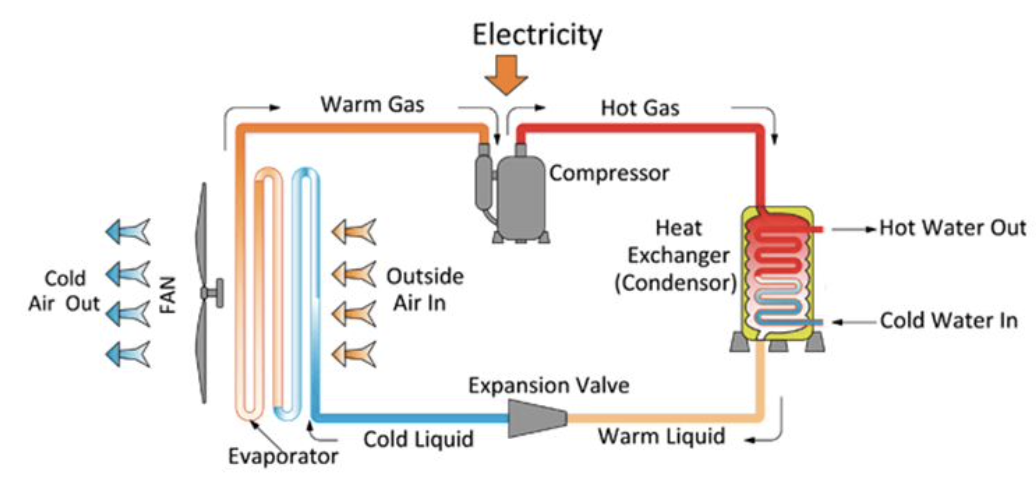
\includegraphics[width=1.1\columnwidth]{Pictures/HPWH_working_principle.png}
        \caption{source:\href{https://inukiengineering.com/heat-pump-water-heaters/}{nukiengineering.com}}
        \label{fig:EWH}
    \end{figure}
I will start with a basic, however, very important thermodynamic principle. \textbf{HEAT ALWAYS GOES TO COLD.} Compressor increases the pressure of the gas passing through to make its temperature very high. This coil goes through the tank which heats up the water inside the tank (top portion). The heat of the gas gets released as it goes down the tank. The output of the tank is the same gas but with less hot temperature. The liquid goes through an expansion valve. The expansion valve "release" the liquid (less pressure therefore less heat) to make the liquid temperature less hot (cold). When the liquid goes through the evaporator, the temperature of the liquid is way less than the outside temperature. Therefore, the cold air gets dumped out and heat comes in. Thus, warm gas goes in to the compressor again and the same cycle is repeated.
\subsection{Coefficient of Performance (CoP)}
In EWH, we measure the efficiency to understand the performance of the WH. However, in the HPWH, we measure the CoP to see the ratio of useful heating or cooling provided to the required work as shown in equation \ref{equ:CoP}. \par
In GridLAB-D waterheater.cpp file, the CoP of the HPWH is defined with an equation that contains a set of integers. To make CoP more accessible, we need a more general equation. 
\begin{equation} \label{equ:CoP}
    CoP = \frac{E_{delivered}}{E_{in}}
\end{equation}
$E_{delivered}$ can be defined as:
\begin{equation}\label{equ:E_delivered}
    \Delta E_{delivered} = \frac{(V_{i}\rho_{w}C_{p,w}(T_{t,i}-T_{ref})) - (V_{i}\rho_{w}C_{p,w}(T_{t-1,i} - T_{ref}))}{t}
\end{equation}
Where:
\begin{itemize}
    \item $V_{i}$ = Volume of the node
    \item $\rho_{w}$ = water density of the node
    \item $C_{p,w}$ = water specific heat capacity.
    \item $T_{t,i}$ = Temperature of the node measured at time t.
    \item $T_{ref}$ = reference water temperature (default)
    \begin{itemize}
        \item For inlet water, the temperature is 60 $\degree$
    \end{itemize}
\end{itemize}
\newpage


\pagebreak
%----------------------------------------------------------------------------------------
%   Section: DCS and CTA-2045
%----------------------------------------------------------------------------------------
\newpage
\section{Summer 2021}
\label{Summer2021}
All data and plots are in PSU Pwrlab Github account. If they're not there, contact midrar@pdx.edu
\pagebreak

% \section{DCS and CTA-2045}
% \label{DCS and CTA-2045}
% \input{DCS and CTA-2045.tex}
% \pagebreak
%----------------------------------------------------------------------------------------
%   Section: EMCB
%----------------------------------------------------------------------------------------

% \newpage
% \section{EMCB Testing}
% \label{EMCB Testing}
% \input{EMCB Testing.tex}
% \pagebreak

%----------------------------------------------------------------------------------------
%   Section: Objectives
%----------------------------------------------------------------------------------------
%\newpage
% \section{Objectives}
% \label{Objectives}
% \input{Objectives.tex}



%----------------------------------------------------------------------------------------
%   Section: Programmable Load Control
%----------------------------------------------------------------------------------------
\newpage
\section{Fall 2021}
\label{Fall2021}
\subsection{Coefficient of Performance: V1}
The coefficient of performance is a measure of the useful energy transferred to the water in the tank per the system's supplied work. In other words, how much thermal energy can one get from 100 W input power, for example. The data obtained from this section are from EMCB use cases. There were different equations obtained from different resources \cite{LeightonClarke}, \cite{Shapiro2016FieldPO}, and \cite{Hudon}. All the aforementioned equations result in the following:
\begin{equation}\label{eq:cop}
    COP = \frac{Q}{E_{input}} = \frac{m \cdot C_{p} \cdot \Delta T}{E_{input}}
\end{equation}
Where:
\begin{itemize}
    \item m is the mass of the water in the tank in Pounds (lbm)
    \item $C_{p}$ is the specific heat of water ($\frac{Btu}{lbm \cdot \circ F}$)
    \item $\Delta T$ is the difference between the ambient temperature and the tank temperature in F.
    \item $E_{input}$ is the electrical power input in Watts. This includes the compressor and the heating element.
\end{itemize}

Equation \ref{eq:cop} is applied to the morning shower in the EMCB studies. The morning shower is a 20 gallon water draw. The change in the water temperature during the heating process is linear. Therefore, a cumulative sum of the input power and then the average were calculated which resulted in 1680 W. Here's a list of the numerical value in equation \ref{eq:cop}:
\begin{itemize}
    \item $E_{input}$ = 1680 W.
    \item m = 50 gallon $\times$ 8.34 = 417 lbm.
    \item C$_{p}$ = 1.001 $\frac{Btu}{lbm \cdot ^{\circ}F}$.
    \item $T_{ambient}$ = 75 $^{\circ}$F
\end{itemize}

For example, if the current temperature in the tank is 100 $^{\circ}F$, then the COP can be calculated as follows:

\begin{equation}
    COP = \frac{(417 [lbm] \times 1.001 \frac{Btu}{lbm \cdot F} \times (100 - 75) [F]) \times 0.293 }{1680 [W]}
    &=1.82
\end{equation}

\begin{figure}[htp!]
    \centering
    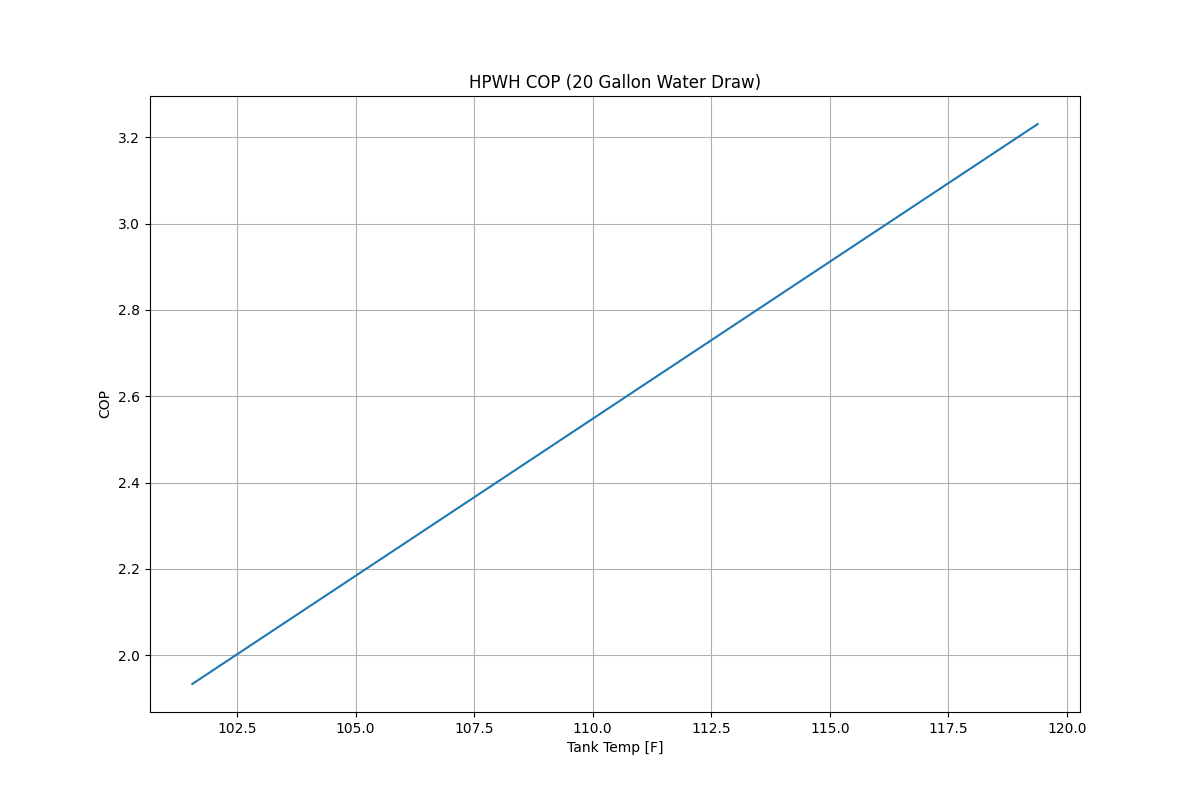
\includegraphics[width=1.1\columnwidth]{Pictures/cop_sim.png}
    \caption{HPWH COP: 20 Gallon Water Draw}
    \label{fig:cop}
\end{figure}
\newpage
\subsection{Coefficient of Performance: V2}
The equation used to calculate and plot the COP of the HPWH is as follows:

\begin{equation}
    COP = \frac{EnergyTake}{Watts}
\end{equation}
The HPWH was set to vacation mode for three days. After, the HPWH was switched to Hybrid mode. Here's the data when the HPWH switch ON.

\begin{longtable}{|l|l|l|}
\hline
time & EnergyTake & Watts  \\ \hline
\endhead
%
Mon Sep 20 12:17:12 2021 &               2775 &       4449.0300 \\ \hline
Mon Sep 20 12:18:12 2021 &               2775 &       4665.8100 \\ \hline
Mon Sep 20 12:19:13 2021 &               2625 &       4686.4500 \\ \hline
Mon Sep 20 12:20:14 2021 &               2550 &       4717.4200 \\ \hline
Mon Sep 20 12:21:14 2021 &               2250 &       4738.0600 \\ \hline
Mon Sep 20 12:22:15 2021 &               2175 &       4748.3900 \\ \hline
Mon Sep 20 12:23:15 2021 &               2025 &       4707.1000 \\ \hline
Mon Sep 20 12:24:16 2021 &               2025 &       4769.0300 \\ \hline
Mon Sep 20 12:25:17 2021 &               1875 &       4769.0300 \\ \hline
Mon Sep 20 12:26:17 2021 &               1800 &       4758.7100 \\ \hline
Mon Sep 20 12:27:18 2021 &               1725 &       4769.0300 \\ \hline
Mon Sep 20 12:28:18 2021 &               1725 &       4769.0300 \\ \hline
Mon Sep 20 12:29:19 2021 &               1650 &       4779.3500 \\ \hline
Mon Sep 20 12:30:19 2021 &               1575 &       4676.1300 \\ \hline
Mon Sep 20 12:31:20 2021 &               1575 &       4707.1000 \\ \hline
Mon Sep 20 12:32:21 2021 &               1425 &       4645.1600 \\ \hline
Mon Sep 20 12:33:21 2021 &               1425 &       4696.7700 \\ \hline
Mon Sep 20 12:34:22 2021 &               1275 &       4696.7700 \\ \hline
Mon Sep 20 12:35:22 2021 &               1200 &       4686.4500 \\ \hline
Mon Sep 20 12:36:23 2021 &               1050 &        392.2580 \\ \hline
Mon Sep 20 12:37:24 2021 &               1050 &        402.5810 \\ \hline
Mon Sep 20 12:38:24 2021 &               1050 &        402.5810 \\ \hline
Mon Sep 20 12:39:25 2021 &                975 &        402.5810 \\ \hline
Mon Sep 20 12:40:25 2021 &                975 &        402.5810 \\ \hline
Mon Sep 20 12:41:26 2021 &                975 &        402.5810 \\ \hline
Mon Sep 20 12:42:27 2021 &                975 &        402.5810 \\ \hline
Mon Sep 20 12:43:27 2021 &                975 &        402.5810 \\ \hline
Mon Sep 20 12:44:28 2021 &                975 &        402.5810 \\ \hline
Mon Sep 20 12:45:28 2021 &                975 &        402.5810 \\ \hline
Mon Sep 20 12:46:29 2021 &                975 &        412.9030 \\ \hline
Mon Sep 20 12:47:29 2021 &                975 &        402.5810 \\ \hline
Mon Sep 20 12:48:30 2021 &                975 &        402.5810 \\ \hline
Mon Sep 20 12:49:31 2021 &                975 &        402.5810 \\ \hline
Mon Sep 20 12:50:31 2021 &                900 &        402.5810 \\ \hline
Mon Sep 20 12:51:32 2021 &                900 &        412.9030 \\ \hline
Mon Sep 20 12:52:32 2021 &                825 &        412.9030 \\ \hline
Mon Sep 20 12:53:33 2021 &                825 &        402.5810 \\ \hline
Mon Sep 20 12:54:34 2021 &                825 &        412.9030 \\ \hline
Mon Sep 20 12:55:34 2021 &                825 &        412.9030 \\ \hline
Mon Sep 20 12:56:35 2021 &                825 &        412.9030 \\ \hline
Mon Sep 20 12:57:35 2021 &                825 &        412.9030 \\ \hline
Mon Sep 20 12:58:36 2021 &                825 &        412.9030 \\ \hline
Mon Sep 20 12:59:36 2021 &                825 &        412.9030 \\ \hline
Mon Sep 20 13:00:37 2021 &                750 &        412.9030 \\ \hline
Mon Sep 20 13:01:38 2021 &                750 &        412.9030 \\ \hline
Mon Sep 20 13:02:38 2021 &                750 &        412.9030 \\ \hline
Mon Sep 20 13:03:39 2021 &                750 &        412.9030 \\ \hline
Mon Sep 20 13:04:39 2021 &                600 &        412.9030 \\ \hline
Mon Sep 20 13:05:40 2021 &                600 &        423.2260 \\ \hline
Mon Sep 20 13:06:41 2021 &                600 &        423.2260 \\ \hline
Mon Sep 20 13:07:41 2021 &                600 &        423.2260 \\ \hline
Mon Sep 20 13:08:42 2021 &                600 &        423.2260 \\ \hline
Mon Sep 20 13:09:42 2021 &                600 &        423.2260 \\ \hline
Mon Sep 20 13:10:43 2021 &                600 &        423.2260 \\ \hline
Mon Sep 20 13:11:43 2021 &                600 &        423.2260 \\ \hline
Mon Sep 20 13:12:44 2021 &                600 &        423.2260 \\ \hline
Mon Sep 20 13:13:45 2021 &                600 &        423.2260 \\ \hline
Mon Sep 20 13:14:45 2021 &                525 &        423.2260 \\ \hline
Mon Sep 20 13:15:46 2021 &                525 &        423.2260 \\ \hline
Mon Sep 20 13:16:46 2021 &                525 &        423.2260 \\ \hline
Mon Sep 20 13:17:47 2021 &                525 &        423.2260 \\ \hline
Mon Sep 20 13:18:48 2021 &                525 &        433.5480 \\ \hline
Mon Sep 20 13:19:48 2021 &                525 &        433.5480 \\ \hline
Mon Sep 20 13:20:49 2021 &                525 &        433.5480 \\ \hline
Mon Sep 20 13:21:49 2021 &                525 &        433.5480 \\ \hline
Mon Sep 20 13:22:50 2021 &                450 &        433.5480 \\ \hline
Mon Sep 20 13:23:51 2021 &                450 &        433.5480 \\ \hline
Mon Sep 20 13:24:51 2021 &                375 &        433.5480 \\ \hline
Mon Sep 20 13:25:52 2021 &                375 &        433.5480 \\ \hline
Mon Sep 20 13:26:52 2021 &                375 &        433.5480 \\ \hline
Mon Sep 20 13:27:53 2021 &                375 &        433.5480 \\ \hline
Mon Sep 20 13:28:53 2021 &                375 &        433.5480 \\ \hline
Mon Sep 20 13:29:54 2021 &                225 &        433.5480 \\ \hline
Mon Sep 20 13:30:55 2021 &                225 &        433.5480 \\ \hline
Mon Sep 20 13:31:55 2021 &                225 &        433.5480 \\ \hline
Mon Sep 20 13:32:56 2021 &                225 &        433.5480 \\ \hline
Mon Sep 20 13:33:56 2021 &                225 &        433.5480 \\ \hline
Mon Sep 20 13:34:57 2021 &                225 &        433.5480 \\ \hline
Mon Sep 20 13:35:58 2021 &                225 &        443.8710 \\ \hline
Mon Sep 20 13:36:58 2021 &                225 &        443.8710 \\ \hline
Mon Sep 20 13:37:59 2021 &                225 &        443.8710 \\ \hline
Mon Sep 20 13:38:59 2021 &                 75 &        443.8710 \\ \hline
Mon Sep 20 13:40:00 2021 &                 75 &        443.8710 \\ \hline
Mon Sep 20 13:41:01 2021 &                 75 &        433.5480 \\ \hline
Mon Sep 20 13:42:01 2021 &                 75 &        433.5480 \\ \hline
Mon Sep 20 13:43:02 2021 &                 75 &        433.5480 \\ \hline
Mon Sep 20 13:44:02 2021 &                 75 &        443.8710 \\ \hline
Mon Sep 20 13:45:03 2021 &                 75 &        443.8710 \\ \hline
Mon Sep 20 13:46:03 2021 &                  0 &        443.8710 \\ \hline
Mon Sep 20 13:47:04 2021 &                  0 &        443.8710 \\ \hline
Mon Sep 20 13:48:05 2021 &                  0 &        443.8710 \\ \hline
Mon Sep 20 13:49:05 2021 &                  0 &        454.1940 \\ \hline
Mon Sep 20 13:50:06 2021 &                  0 &        443.8710 \\ \hline
Mon Sep 20 13:51:06 2021 &                  0 &        454.1940 \\ \hline
Mon Sep 20 13:52:07 2021 &                  0 &        454.1940 \\ \hline
Mon Sep 20 13:53:07 2021 &                  0 &        454.1940 \\ \hline
Mon Sep 20 13:54:08 2021 &                  0 &        443.8710 \\ \hline
Mon Sep 20 13:55:08 2021 &                  0 &        454.1940 \\ \hline
Mon Sep 20 13:56:09 2021 &                  0 &        454.1940 \\ \hline
Mon Sep 20 13:57:09 2021 &                  0 &        454.1940 \\ \hline
Mon Sep 20 13:58:10 2021 &                  0 &        454.1940 \\ \hline
Mon Sep 20 13:59:11 2021 &                  0 &        454.1940 \\ \hline
Mon Sep 20 14:00:11 2021 &                  0 &        454.1940 \\ \hline
Mon Sep 20 14:01:12 2021 &                  0 &        454.1940 \\ \hline
Mon Sep 20 14:02:12 2021 &                  0 &        454.1940 \\ \hline
Mon Sep 20 14:03:13 2021 &                  0 &        454.1940 \\ \hline
Mon Sep 20 14:04:13 2021 &                  0 &        454.1940 \\ \hline
Mon Sep 20 14:05:14 2021 &                  0 &        464.5160 \\ \hline
Mon Sep 20 14:06:15 2021 &                  0 &        454.1940 \\ \hline
Mon Sep 20 14:07:15 2021 &                  0 &        454.1940 \\ \hline
Mon Sep 20 14:08:16 2021 &                  0 &        454.1940 \\ \hline
Mon Sep 20 14:09:16 2021 &                  0 &        454.1940 \\ \hline
Mon Sep 20 14:10:17 2021 &                  0 &        454.1940 \\ \hline
Mon Sep 20 14:11:17 2021 &                  0 &         41.2903 \\ \hline
Mon Sep 20 14:12:18 2021 &                  0 &         30.9677 \\ \hline
Mon Sep 20 14:13:19 2021 &                  0 &         41.2903 \\ \hline
Mon Sep 20 14:14:19 2021 &                  0 &         41.2903 \\ \hline
Mon Sep 20 15:20:57 2021 &                  0 &         10.3226 \\ \hline

\end{longtable}

The HPWH was ON for 81 minutes to heat the water up to the setpoints, 120 $^{\circ}F$. Therefore, the values of watts consumed was converted to Watts-hour as follows:
\begin{equation}
    Wh = Watts \times \frac{x-1}{60}
\end{equation}
Where x is the duration of the heating process.

The following figures show the COP VS:
\begin{itemize}
    \item time
    \item EnergyTake
    \item Line fit
\end{itemize}
\textbf{The average COP is 3.2}

\begin{figure}[htp!]
    \centering
    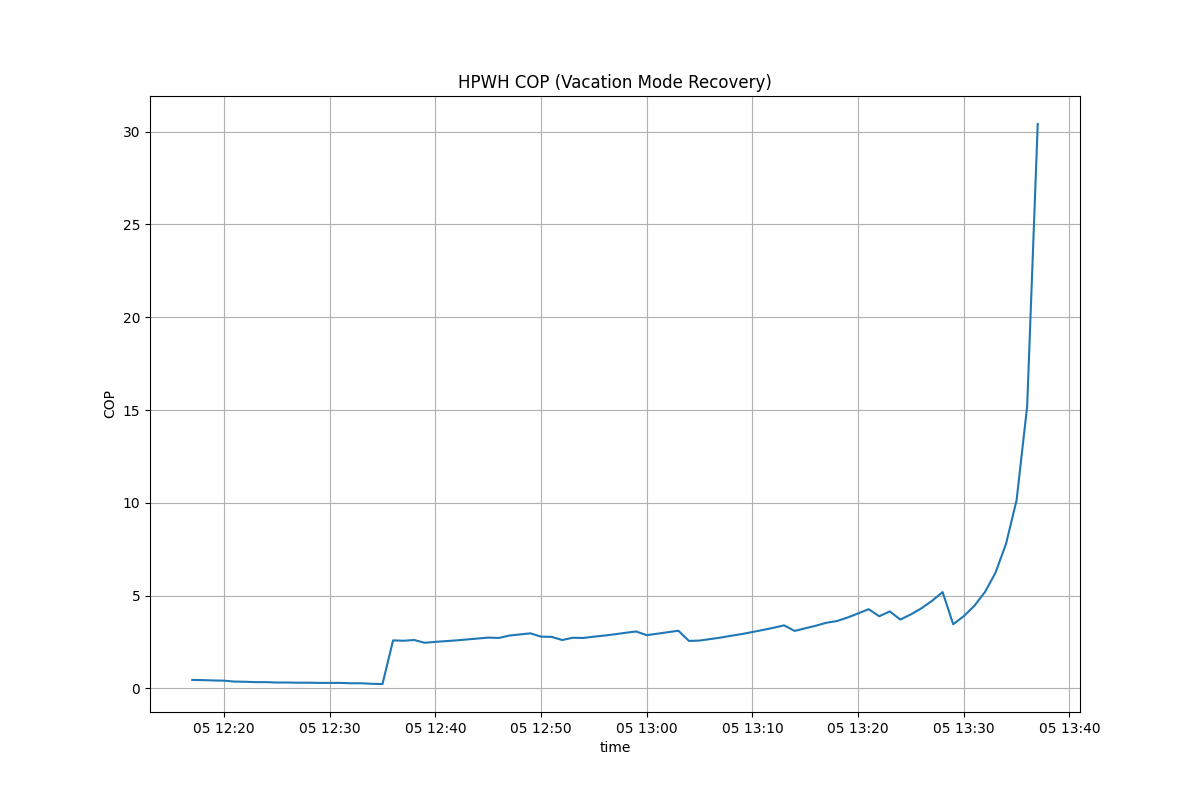
\includegraphics[width=1.1\columnwidth]{Pictures/cop_vs_time.png}
    \caption{HPWH COP vs Time: Vacation Mode Recovery}
    \label{fig:copvstime}
\end{figure}

\begin{figure}[htp!]
    \centering
    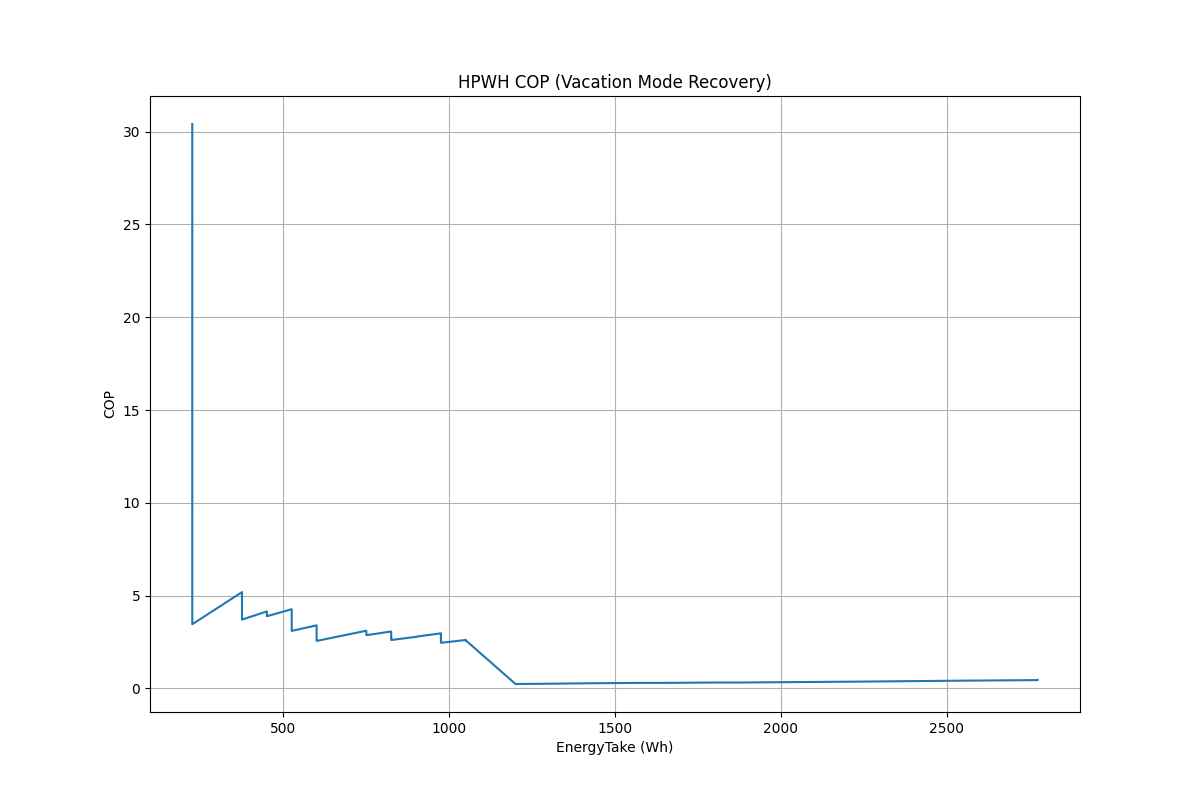
\includegraphics[width=1.1\columnwidth]{Pictures/cop_vs_EnergyTake.png}
    \caption{HPWH COP vs EnergyTake: Vacation Mode Recovery}
    \label{fig:copvsenergytake}
\end{figure}
\newpage

\subsection{this should work in a good position}

%----------------------------------------------------------------------------------------
%    APPENDICES
%----------------------------------------------------------------------------------------
%\newpage
%\appendix

%\section{Appendix: NameMe}
%\label{AppNameMe}
%\input{App_NameMe}
%\pagebreak

%----------------------------------------------------------------------------------------
%	BIBLIOGRAPHY
%----------------------------------------------------------------------------------------
\newpage
\bibliographystyle{unsrt}%Used BibTeX style is unsrt
\bibliography{bibfile}

% \cite{R01}
% \cite{R02}
% \cite{NFPA70}
% \cite{R04}
% \cite{R05}
% \cite{R06}
% \cite{IEEETEST}
% \cite{loads_wiki}
% \cite{resloads_wiki}
% \cite{app_wiki}
% \cite{evcharger_wiki}
% \cite{ZIPload}
% \cite{R10}
% \cite{R11}
% \cite{RECS}
% \cite{NC_web}


%----------------------------------------------------------------------------------------
%----------------------------------------------------------------------------------------
%    Section: Authors, Lab, Disclaimer & Acknowledgements
%----------------------------------------------------------------------------------------
\newpage
\input{Bios}
\pagebreak
%----------------------------------------------------------------------------------------

\end{document}
